\documentclass[main.tex]{subfiles}
\begin{document}
\onlyinsubfile{\mainmatter{}}

\chapter{Sealed Objects} \label{ch:obj}
The previous chapter discusses a first extension of the Glyco compiler, namely a secure calling convention. This chapter treats a second extension, a feature we call \emph{sealed objects}.

Sealed objects depend on two new features; we begin hence by describing lambdas in \cref{sct:lambda} and named \& nominal types in \cref{sct:named-ty} before defining the semantics of objects and methods in \cref{sct:obj-meth}. We then list in \cref{sct:obj-sec} a few security properties afforded by sealed objects. We finish this chapter by evaluating the changes to the compiler in \cref{sct:obj-eval}.

This chapter discusses the feature set and languages of Glyco 0.3.\footnote{The source code is available at \url{https://tsarouhas.eu/glyco/0.3/}.} A full language reference can be found in \cref{ch:grammar}.

\section{Lambdas} \label{sct:lambda}
A first addition to Glyco is the \textbf{lambda}, i.e., an anonymous function, in a new \g{il} called \textbf{Λ} (Lambdas) above EX. Lambdas allow the programmer to define functions (\texttt{λ} values) at the point of use and to pass them around as values. For example, the Λ program in \cref{lst:sum} defines a lambda that computes the sum of its two parameters and immediately applies it on $1080$ and $-80$.
\begin{listing}[ht]
	\ilfile{Programs/sum.l}
	\caption{A Λ program evaluating to 1000.}
	\label{lst:sum}
\end{listing}

The scope of a lambda definition extends beyond the \texttt{λ} value itself to the \texttt{let} value defining it, in a similar way to \texttt{letRec} values in some functional programming languages and unlike definitions of other kinds of values. This enables mutual recursion such as the (inefficient) program in \cref{lst:mutrec} determining the parity of 420.
\begin{listing}[ht]
	\ilfile{Programs/evenodd.l}
	\caption{A Λ program featuring mutual recursion.}
	\label{lst:mutrec}
\end{listing}

Finally, since \texttt{λ} values with support for mutual recursion provide the same expressive power as programs with global functions, Λ removes support for global functions. The reader should bear in mind however that lambdas do not \emph{increase} the (practical) expressive power of programs but merely make it easier to define functions. Lambda values evaluate to code capabilities and do not carry an environment, i.e., lambdas in Λ are not closures.\footnote{Spoiler alert: \Cref{ch:cls} introduces closures.}

\paragraph{From Λ to EX} The \g{nanopass} from Λ to EX extracts the functions defined by \texttt{λ} values into the global scope (with either an auto-generated name or a name derived from the lambda definition) and replaces the \texttt{λ} values by code capabilities to those functions. The program in \cref{lst:sum} is thus \lowered{} to the EX program
\ilfile{Programs/sum.ex}

The \g{nanopass} also injects all λ values in the same \texttt{let} value in the lambda body to enable (mutual) recursion. The parity program in \cref{lst:mutrec} is thus \lowered{} as
\ilfile{Programs/evenodd.ex}

\section{Alias \& Nominal Types} \label{sct:named-ty}
A second new feature is support for defining new (\textbf{named}) \textbf{types} in a new \g{il} \textbf{NT} (Named Types) above Λ. A value in NT can be
\begin{itemize}[nosep]
	\item an (8-bit) byte, a \iil/u8/;
	\item a (32-bit) signed integer, an \iil/s32/;
	\item a capability to a vector of \iil/T/s, a \iil/cap(vector(T, sealed: S))/;
	\item a capability to a record, a \iil/cap(record((name, Type) …, sealed: S))/;
	\item a capability to a function, a \iil/cap(function(takes: p …, returns: r))/;
	\item a \g{sealcap}, a \iil/cap(seal(sealed: S))/; or
	\item a value of a type named \iil/T/
\end{itemize}
where \iil/S/ is \iil/true/ if the capability is sealed and \iil/false/ otherwise. A type can be defined using a \textbf{\texttt{letType} value} in one of two ways.

\paragraph{Alias types} An \textbf{alias type definition} creates an \textbf{alias type}, a type that is equivalent to the type it's defined as. An alias type can have a shorter or semantically meaningful type name that the type it's defined as.

For instance, the following NT program defines an alias type named \iil/Sequence/ and uses it in a simple computation that evaluates to 4. The value \iil/pi/ created by \iil/vector(0, count: 3)/ is typed \iil/cap(vector(s32, sealed: false))/ but is accepted by the function which takes an argument typed \iil/Sequence/.
\ilfile{Programs/alias.nt}

\paragraph{Nominal types} A \textbf{nominal type definition} creates a \textbf{nominal type}, a type which is only equivalent to itself. A nominal type is effectively a new type by itself and can be used to ensure that values of two representationally identical but semantically different types cannot accidentally be mixed. However, a value can be explicitly \texttt{cast}ed to a value of a different type that has the same representation.

For example, the following NT program defines two nominal types \iil/Kelvin/ and \iil/Celsius/ and uses them to convert 500 °C to K and back to °C.
\ilfile{Programs/temp.nt}

However, the following program is not valid since the second invocation of \iil/toCelsius/, which expects a value in \iil/Kelvin/, is given a value in \iil/Celsius/. Nominal type rules prevent the accidental conversion from \iil/Kelvin/ to \iil/Celsius/, even though both types are represented by \iil/s32/.
\ilfile{Programs/tempbad.nt}

\begin{quote}
	\ttfamily\footnotesize
	Error: \iil/evaluate(toCelsius, 500)/ is of type \iil/named(Celsius)/ and thus cannot be used for \iil/(k, Kelvin)/
\end{quote}

\paragraph{Implicit type casts} With some exceptions, the type checker rejects any uses of values of a structural type such as \iil/s32/ in contexts where a nominal type is expected and vice versa. This restriction can be bypassed using a \texttt{cast}. For ergonomic reasons, the type-checker performs an implicit cast on
\begin{itemize}[nosep]
	\item an argument of structural type that is passed to a parameter of nominal type, like in \iil/evaluate(toKelvin, 500)/ above;
	\item a record value of nominal type in a \texttt{field} value;
	\item a vector value of nominal type in an \texttt{element} value;
	\item a seal value of nominal type in a \texttt{sealed} value;
	\item an operand of structural type in a \texttt{binary} value when the other operand is of nominal type — the result of the \texttt{binary} value is in that case of nominal type;
	\item a lambda's result value of structural type when the result type is nominal; and
	\item a program's result value of nominal type (to \iil/s32/), like the result in \iil/Celsius/ above.
\end{itemize}

\paragraph{From NT to Λ} The \g{nanopass} from NT to Λ replaces named types by their Λ equivalents and checks if the nominal typing rules hold.

\section{Objects \& Methods} \label{sct:obj-meth}
Objects in object-oriented programming languages are constructs that consist of state and behaviour. An object owns a region of memory where it holds its state while its behaviour manifests through its methods, which are functions that access and modify the object's state as part of their operation.

Objects usually provide encapsulation, a technique that discourages or prohibits code outside of an object's method from accessing or modifying the object's state, thereby promoting the decoupling of disparate parts of a codebase. For instance, the following NT program implements a \iil/Counter/ type, which is a record consisting of a single integer value, and two lambdas that return resp. increase the counter's value. It then creates a \iil/Counter/ with an initial value of 32 which it then increases three times.
\ilfile{Programs/unsealedcounter.nt}

In this NT program, \iil/counter/ is an \enquote{object} and \iil/increaseCounter/ and \iil/getCounterValue/ are the \enquote{methods} which access or modify the \iil/counter/'s state. However, nothing prevents from external code from directly accessing the \iil/value/ field, for example to \emph{decrease} it — \iil/Counter/ objects are not encapsulated.

\paragraph{Sealed objects \& methods} A \textbf{sealed object} (or simply \textbf{object} in this chapter) is an encapsulated record (the object's \textbf{state}) on which a predetermined set of methods can be invoked. A \textbf{method} is a function that (among other parameters) takes a capability to an object's state. We refer to the object on which a method is called as the method's \textbf{receiver}.

\paragraph{Object types \& initialisers} An object belongs to an \textbf{object type}, which determines the record type and \gs{method} of all objects of that type. Object types in Glyco are in this respect similar to classes in programming languages such as Java. Object types however do not support inheritance and record fields cannot be made visible outside of \gs{method}.

Object types can be defined in a new \g{il} above NT called \textbf{OB} (Objects) using an \textbf{object type definition} in a \texttt{letType} value. A definition consists of
\begin{itemize}[nosep]
	\item a name, like any other type definition;
	\item a record type specifying the structure of each object's state;
	\item an initialiser effect applied on all new objects accepting zero or more parameters; and
	\item zero or more \gs{method}.
\end{itemize}

An \textbf{\g{init}} is a pseudo-\g{method} automatically invoked on every new object immediately after its state is allocated that ensures that the object has the right initial state. An object can be created using an \texttt{object} value, which accepts a type name and arguments to the initialiser's parameters. \Gs{method} can only be defined when the object type is being defined. They can be invoked using a \texttt{message} value, which takes an object, \g{method} name, and arguments to the \g{method}'s parameters. Initialisers and \gs{method} alike get a capability to the object's state, i.e., the record composing it, through the \iil/self/ value.

The OB program in \cref{lst:counter} reimplements the \iil/Counter/ type as an object type, creates a counter with an initial value of 32, increases the count three times, and evaluates to the counter's final value (35).
\begin{listing}[ht]
	\ilfile{Programs/counter.ob}
	\caption{An OB program implementing a counter and counting from 32 to 35. The \iil/evaluate(message(counter, increase),)/ syntax is valid in Glyco 1.0 and is introduced in the next chapter. The equivalent syntax in this chapter's version (Glyco 0.3) is \iil/message(counter, increase,)/. Additionally, initialisers in Glyco 0.3 receive a pre-allocated record in \iil/self/ while initialisers in the final version (shown here) allocate themselves a record.}
	\label{lst:counter}
\end{listing}

\subsection{Object State Encapsulation \& Unique Seals} \label{sct:obj-sec}
The first important security property afforded by sealed objects, the \textbf{encapsulation property}, is that an object's state is \textbf{only accessible within the \g{init} or a \g{method} defined during object type definition} in \texttt{letType}.\footnote{This property does not hold if the \g{init} or a \g{method} leaks an unsealed capability to the state record. Our threat model assumes trust in an object type's implementation.} A second security property is that a \g{method} or \g{init} \textbf{can only be invoked on an object of the type defining that \g{method} or \g{init}}.\footnote{This property similarly does not hold if an unsealed code capability to the \g{method} is leaked by the type owner.}

Both properties are achieved by \g{sealing} capabilities to objects and \gs{method} using unique \gs{sealcap} provided by a \g{rtrt}. \G{sealing} capabilities using a \g{sealcap} is a power which was originally bestowed upon the \g{rt} in the design and implementation of \g{ghscc} where an \g{scall} seals a return–frame capability pair before passing control to the callee.

An \textbf{\g{objcap}} is a sealed capability to a record embodying an object. A \textbf{\g{methcap}} is a sealed code capability to a \g{method}. Due to their sealed nature, \gs{objcap} cannot be used in an \texttt{getField} value or \texttt{setField} effect and similarly \gs{methcap} cannot be used in an \texttt{evaluate} value without a receiver of the right object type.\footnote{A \texttt{getField} value is eventually \lowered{} to a load instruction in the CHERI-RISC-V language. A \texttt{setField} effect is eventually \lowered{} to a store instruction. An \texttt{evaluate} value is eventually \lowered{} to either a \texttt{CJALR} or \texttt{CInvoke} instruction. Loading or storing using a sealed capability, jumping to a sealed code capability using \texttt{CJALR}, or invoking a mismatched code–data capability pair using \texttt{CInvoke} results in a machine trap.}

Object and method capabilities belonging to the same object type are sealed using the same \g{sealcap}; a \g{methcap} can therefore be invoked on an \g{objcap} using the \texttt{CInvoke} CHERI-RISC-V instruction. A \g{methcap} cannot be invoked on an \g{objcap} belonging to a different object type; the hardware ensures this invariant when the \texttt{CInvoke} instruction is executed, with a violation causing a machine trap.

\subsection{Object Types Are Objects}
When an object type is defined in a \texttt{letType} value, a unique \g{sealcap} is created and used for sealing the new type's \gs{methcap}. This capability must be protected from adversaries as it allows for additional methods to be defined. With access to the \g{sealcap}, the adversary merely needs to seal a \g{methcap} of its own and invoke the adversarial method on the sealed object to get access to the object's state, thereby breaking the encapsulation property.

An object type's \g{sealcap} is also needed for sealing new \gs{objcap}, i.e., for creating new objects of the object type. To allow an adversary to create new objects of a type it does not own, Glyco introduces the concept of an \textbf{object type object}, an object representing an object type, and the notion of a \textbf{metatype}, the type of a type object. The metatype provides a \texttt{createObject} method with the same parameters as those of the type's \g{init} and which produces an \g{objcap}. The \g{sealcap} needed for \g{sealing} the capability to the initialised state of the new object is stored within the type object and only accessible from within the \texttt{createObject} method by relying on the security properties afforded by objects.

Each object type has an associated type object and metatype. The metatype (the type object's type) does not define an \g{init}; instead, the singleton type object's state is statically allocated and initialised at the point of the object type definition and the metatype's \g{sealcap} is discarded after use.

\subsection{\G{lowering} OB to NT}
We'll work through the OB to NT \g{nanopass} by applying it on the \iil/Counter/ example in \cref{lst:counter}.
\ilfile[lastline=2]{Programs/counter.nt}

An object type definition (in a \texttt{letType}) is \lowered{} to NT by
\begin{enumerate}[nosep]
	
	\item defining a nominal type definition;
	\ilfile[firstline=3, lastline=5]{Programs/counter.nt}
	
	\item creating unique \gs{sealcap} for the metatype and the new type;
	\ilfile[firstline=6, lastline=7]{Programs/counter.nt}
	
	\item allocating and initialising a type object with the type's \g{sealcap};
	\item sealing the capability to this object with the metatype's \g{sealcap};
	\ilfile[firstline=8, lastline=14]{Programs/counter.nt}
	
	\item implementing the metatype's \texttt{createObject} method using a lambda that allocates a state record, executes the initialiser's effect, seals a capability to the state record using the \g{sealcap} stored in the type object, and returns this sealed capability to the method's caller;
	\item sealing the capability for this method with the metatype's \g{sealcap};
	\ilfile[firstline=15, lastline=33]{Programs/counter.nt}
	
	\item implementing each method of the type using a lambda that takes a sealed parameter \iil/ob.self/ representing the receiver (and which the \iil/self/ value maps to) plus any parameters defined on the method; and finally,
	\item sealing the capability of each of the type's methods.
	\ilfile[firstline=34, lastline=69]{Programs/counter.nt}
	
\end{enumerate}

Each method invocation is \lowered{} by evaluating the \g{methcap} with the receiver as the first argument, followed by any provided arguments. Object construction in \texttt{object} values is implemented in NT by calling the metatype's \texttt{createObject} \g{methcap} on the type object.
\ilfile[firstline=70]{Programs/counter.nt}

\section{Evaluation: Impact on the Codebase} \label{sct:obj-eval}
Similarly to what we did in \cref{sct:ghscc-eval}, we evaluate the impact of the implementation of sealed objects in Glyco. The changes to the compiler pipeline are also summarised in \cref{fig:pipeline03}.

\begin{figure}
	\centering
	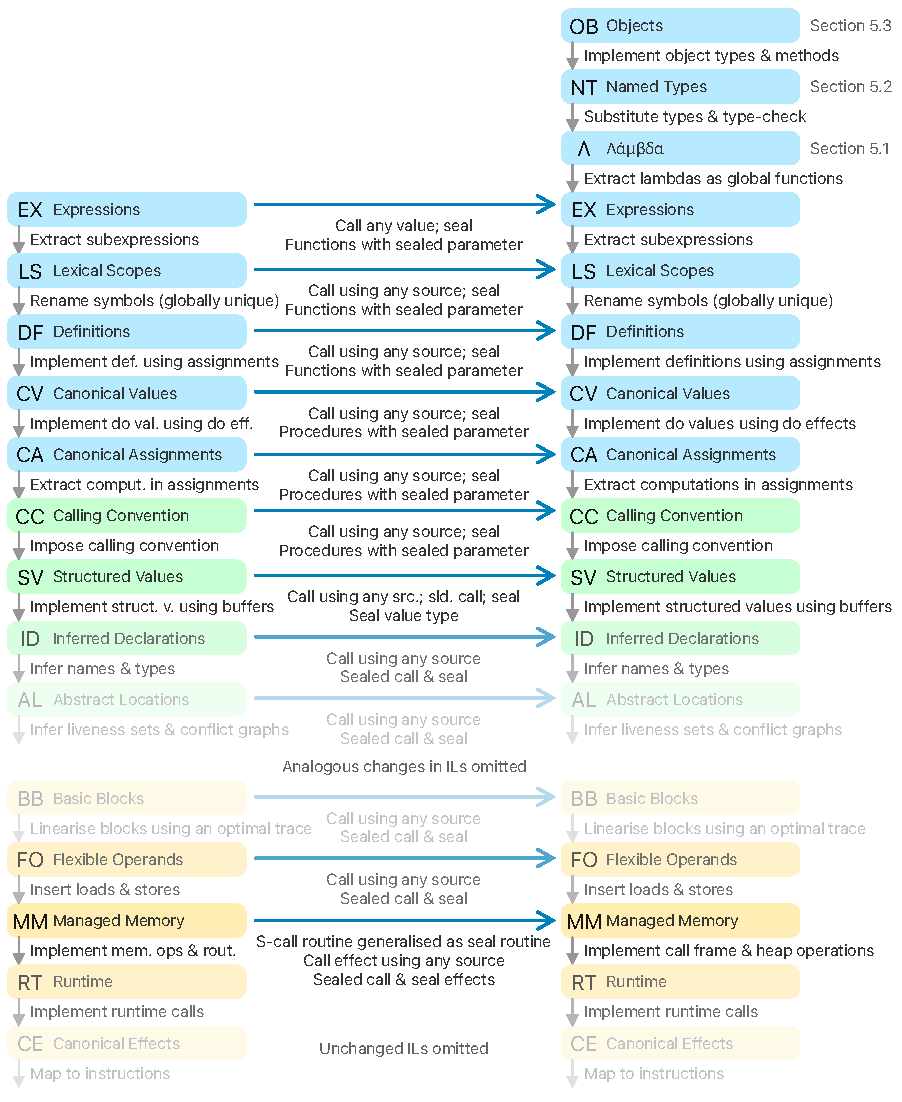
\includegraphics{Images/Pipeline v0.3.pdf}
	\caption{The Glyco 0.2 (left) and 0.3 (right) pipelines and the main differences between them.}
	\label{fig:pipeline03}
\end{figure}

\paragraph{Managed Memory (MM)} The \g{scall} \g{rtrt} is generalised to a seal allocation routine, given that both \g{scall} and object type definition only need a \g{rtrt} to securely provide a unique \g{sealcap} for next invocation resp. object type definition. The language now provides new \texttt{createSeal} and \texttt{seal} effects. The \texttt{call} effect's \g{lowering} under \g{ghscc} is modified to invoke the seal allocation routine and use the returned \g{sealcap} to seal the return–frame capability pair.

A \texttt{callSealed} effect is also added to the \g{il}'s syntax which performs roughly the same as the \texttt{call} effect, except that it accepts a sealed code–data capability pair, as required for method invocation.

\paragraph{Flexible Operands (FO)} The \texttt{createSeal}, \texttt{seal}, and \texttt{callSealed} effects from MM are propagated to FO. Just like for other FO effects, the FO to MM \g{nanopass} inserts any required loads and stores around the underlying MM effect.

The \texttt{call} effect is updated to accept any kind of source, not just labels. This is needed to enable calling code capability values, which is how lambdas are represented across the compiler pipeline.

\paragraph{Basic Blocks (BB) and Predicates (PR)} The \texttt{createSeal}, \texttt{seal}, and updated \texttt{call} effects from FO are propagated to BB and PR. A new \texttt{callSealed} continuation is added.

\paragraph{Conditionals (CD) through Structured Values (SV)} The 3 new effects and updated \texttt{call} effect are propagated through these 5 \gs{il}, usually with a trivial \gs{lowering}.

\paragraph{Structured Values (SV)} An additional \g{sealcap} value type is added. The \texttt{createSeal} effect creates capabilities of this type while the \texttt{seal} effect uses them.

\paragraph{Calling Convention (CC)} The \texttt{createSeal}, \texttt{seal}, and updated \texttt{call} effects from SV are propagated to CC but the \texttt{callSealed} effect is not. Instead, individual parameters can now be marked as being sealed. The \texttt{call} effect is lowered using a \texttt{call} resp. \texttt{callSealed} effect in SV when the target procedure has zero resp. one sealed parameter(s). CC does not support calling procedures with two or more sealed parameters.\footnote{One way to implement support for such procedures is to transform each procedure taking multiple sealed parameters to first call itself multiple times, each time unsealing a different argument.}

\paragraph{Canonical Assignments (CA)} The \texttt{createSeal} and \texttt{seal} effects from CC as propagated to CA as sources. The \texttt{call} effect is updated to accept any kind of source for its procedure operand instead of only accepting labels.

\paragraph{Computed Values (CV) through Expressions (EX)} The \texttt{createSeal} and \texttt{seal} sources from CA as propagated to CV, DF, LS, and EX as values. The evaluate value is similarly updated to accept any kind of source for its procedure operand.

\paragraph{Lambdas (Λ) through Objects (OB)} These new \gs{il} are described in the preceding sections.

\paragraph{Codebase growth} The implementation of lambdas, named types, and sealed objects introduces 3 new \gs{il} (Λ, NT, and OB) bringing the total in Glyco 0.3 to 22 \gs{il}. Using cloc again, we measured a growth in the codebase from 6921 SLOC in Glyco 0.2 to 9360 SLOC in Glyco 0.3, representing a net growth of $+35\%$. However, as noted in \cref{sct:ghscc-eval}, a significant part of this growth is due to code duplication.

\onlyinsubfile{\glsaddall\printglossaries}
\end{document}
